\section*{Related Work}

A complex system with individuals interacting with one another according to certain rules, at the macro level, exhibits a totally different function which the sum of all individual functions does not possess (such as structure of time, space, and function), known as emergence, resulting in emergent behavior [17]. This model can be identified as a major interest in the development of swarm intelligence, as the evolution in functionality promotes a higher degree of adaptability, security, and effectiveness. In this heuristic design space, it is required that the intelligence factor exhibit any dimension of emergent behavior for it be considered swarm intelligence and possess the value as stated in previous sections. In this section, we outline past and current work towards the development of swarm intelligence that experiences emergent behavior. The literature on these multi-agent systems details numerous tools and algorithms for coordinated motion, formation control, consensus, rendezvous, and flocking which highlights the advancements of swarming behavior.


Given that emergent behavior of a swarm derives inspiration from natural social systems, it is important to understand the root of swarming intelligence and how these systems organically evolve towards optimal performance. Much of this can be attributed to metaheuristics, which are algorithms derived from the behavior of social insects, flocks of birds, and fish schools []. These natural social systems Yang et al. derives the relationship between metaheuristics and swarm intelligence, and how these behavioral models have been extensively investigated through the development and application of algorithms that could best represent the possibility self-organization. Certain conditions are necessary for systems to self-organize feedback, stigmergy (when individual system parts intercommunicate indirectly by modifying their local environment), multiple interactions, memory, and environmental setting [18, 20]. These characteristics can be replicated using both deterministic and stochastic algorithms, with each having their own drawbacks and limitations []. A representation of a self-organized system at the smallest of scale can be observed in a particle system, illustrated in Figure 3.

\begin{figure}[!h]
  \centering
  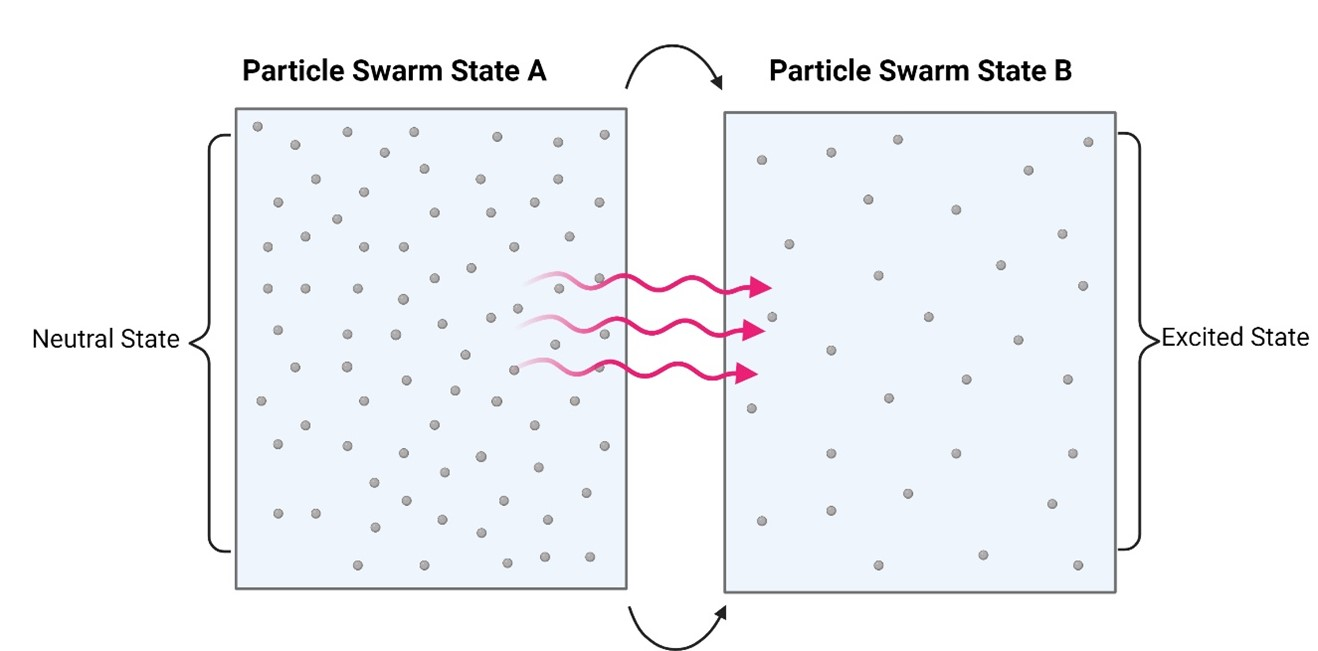
\includegraphics[width=0.7\textwidth]{particles.jpg}
  \caption{Diagram of a standard particle system, which undergoes self-organization due to the experience of an external stimulus, that causes the system to transition from a neutral state to an excited state. }
  \label{fig:platforms}
\end{figure}

A fundamental example of self-organized behavior can be seen in a typical particle system. Generally, the particle agents in amass exist in a neutral state, until introduced to an external stimulus. At this instance, the particles assume an excited state, in which they separate or reorganize in accordance with the magnitude and direction of the perceived stimulus. Such a response can also relate to the attributes of the particles (composition, polarity, size, etc.). This phenomenon can be correlated to that of a flock of birds, who fly in accordance with the group’s speed and direction until an anticipated external factor, such as a predator, which results in a change in direction and individual distance. Some typical natural self-organized systems are detailed below in Table 2. Characteristics of each organic system plays an important role in identifying the overall intention of such entities and their purpose of acting within a swarm model.

\begin{table}[]
\footnotesize{
\begin{tabular}{p{1cm}p{1cm}p{3.5cm}p{3.5cm}p{3.5cm}p{1cm}}
% {cccccc}
\hline
Swarm Entity & System Agents & Common Objectives & Interaction Mechanism & Optimized Parameters & Ref. \\ \hline
School & Fish & Protection from predators, improved foraging,   reproduction, and efficient swimming & Vibration detection, spatial coordination, and   changes in water currents & Coordination, survival, and preservation & {[}53{]} \\ 
\hline
Colony & \begin{tabular}[c]{@{}c@{}}Ants\\    \\ Bees\end{tabular} & Foraging, nest development, and protection & Pheromones & Coordination path, danger aversion, and target   profit & {[}54{]} \\ 
\hline
Flock & Birds & Protection from predators, long-distance migrations & Motion of neighbors, biological radios (calls), visual cues & Coordination path, and spent energy & {[}55{]} \\ 
\hline
Cauldron & Bats & Increased reproductive success & Echolocation, body movements & Preservation, acquisition of food & {[}56{]} \\ 
\hline
Pack & Wolves & Food acquisition, territory & Sound, smell, and body language & Preservation, acquisition of food & {[}57{]} \\ 
\hline
Raft & Penguins & Protection from predators, warmth & Vocal and visual displays & Survival, nesting territories, partner, and chick recognition & {[}58{]} \\ \hline
System & Particles & Molecule construction & Inter-atomic forces, polarities & Complexity of matter, low-energy molecules, etc. & {[}59{]} \\ 
\hline
\end{tabular}}
\caption{Examples of typical natural social systems that reflect a self-organized entity with specific interaction mechanisms and target parameters to optimize from collaboration.}
\label{tab:my-table}
\end{table}